\documentclass{article}
\usepackage{tikz,times}
\usepackage[paperwidth=25cm,paperheight=22cm,left=1cm,top=1cm]{geometry}

\usetikzlibrary{mindmap,backgrounds}

\pagestyle{empty}

\begin{document}
\centering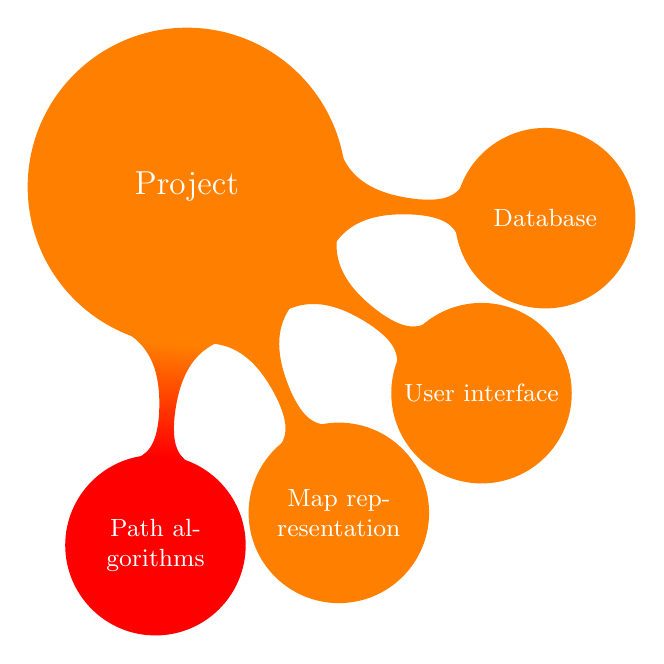
\begin{tikzpicture}[mindmap,
  level 1 concept/.append style={level distance=130,sibling angle=30},
  extra concept/.append style={color=blue!50,text=black}]

  % C++

  \begin{scope}[mindmap, concept color=orange, text=white]
    \node [concept] {Project}[clockwise from=-5] 
      child {node [concept] (db) {Database}}
	  child {node [concept] (ui) {User interface}}
      child {node [concept] (mr) {Map representation}}
      child [concept color=red] {node [concept] (pa) {Path algorithms}};
  \end{scope}





\end{tikzpicture}

\end{document}